\subsection{Chiral Magnetic Effect}

%\begin{itemize}
%	\item
%The vacuum of quantum chromodynamics (QCD) is characterized by rich geometry structure which may corresponds to the fractal-like geometry \cite{IJMPE-22-1350041-2013}.There is a fundamental interrelation between geometry and essential properties of QCD Lagrangian.Structures with non-trivial topology in QCD vacuum are believed to determine the behavior of the $\mathcal{P / CP}$ fundamental symmetries in the hot quark-gluon matter. Due to higher luminosity at the HL--LHC and / or high multiplicity per event at HE--LHC energy the multiparticle azimuthal correlations can be used for investigations of wide set of chiral effects in strong interaction \cite{PAN-80-1133-2017}, for instance, chiral magnetic effect -- CME, chiral magnetic waves -- CMW etc. This approach  allows the significant suppression of the backgrounds and improvement of reliability of physical conclusions. The study of charge-dependent azimuthal correlations for various types of light flavor particles can be possible with unprecedented precision due to high luminosity of the HL--LHC project. Consequently the quantitative comparison will be allowed for strengths of correlations in meson, baryon--meson and baryon systems. Such measurements will be essential in particular for search for chiral vortical effect -- CVE and its study with high precision. Furthermore the higher energies of the HE--LHC project can provide the opportunity for study of flavor dependence of the $\mathcal{P / CP}$ violation with help the azimuthal correlations for wider set of types of secondary particles including for heavy flavor ones. Thus experimental study of topology of QCD vacuum can be one of the focuses for studies of bulk properties within the HL--LHC, HE--LHC projects.
%\end{itemize}

An important property of the strong interaction which is potentially observable in heavy-ion collisions is parity violation. Although it is allowed by 
quantum chromodynamics (QCD), global parity violation is not observed in strong interaction. However, QCD predicts the existence of topologically 
non-trivial configurations of the gluonic field, instantons and sphalerons, which might be responsible for local parity violation in microscopic QCD 
domains at finite temperature \cite{Lee:1973iz, Lee:1974ma, Morley:1983wr, Kharzeev:1998kz}. The $P$- and $CP$-odd interactions between quarks 
and such fields with non-zero topological charge~\cite{Chern:1974ft} change the quark chirality, breaking parity symmetry by creating an imbalance 
between the number of left- and right-handed quarks. Furthermore, an extremely strong magnetic field is expected to be produced in heavy-ion collisions 
\cite{Deng:2012pc, Gursoy:2014aka} (of the order of $10^{19}$ Gauss at the LHC) because the charges of initial ions add coherently. This strong 
magnetic field aligns the spins of the negatively (positively) charged quarks in the direction anti-parallel (parallel) to magnetic field orientation. Moreover, 
right-handed (left-handed) quarks have their direction of momentum parallel (anti-parallel) to the spin orientation. The spin alignment coupled with the 
local imbalance between the number of left- and right-handed quarks leads to the development of a quark current. The current moves the positively 
charged quarks along its direction and the negatively charged quarks in the opposite direction. This implies a charge separation along the direction 
of the magnetic field, which is on average perpendicular to the symmetry plane (defined by the participant nucleons and the beam direction), a 
phenomenon called Chiral Magnetic Effect (CME) \cite{Kharzeev:2004ey, Kharzeev:2007tn, Kharzeev:2007jp, Fukushima:2008xe}. 

Since the sign of 
the topological charge is equally probable to give rise to a positive or negative current in the magnetic field direction, the charge separation averaged 
over many events is zero. This makes the observation of the CME experimentally difficult and possible only via azimuthal particle correlations, which 
introduces a large flow related background into the measurements.

\begin{figure}[!ht]
\begin{center}
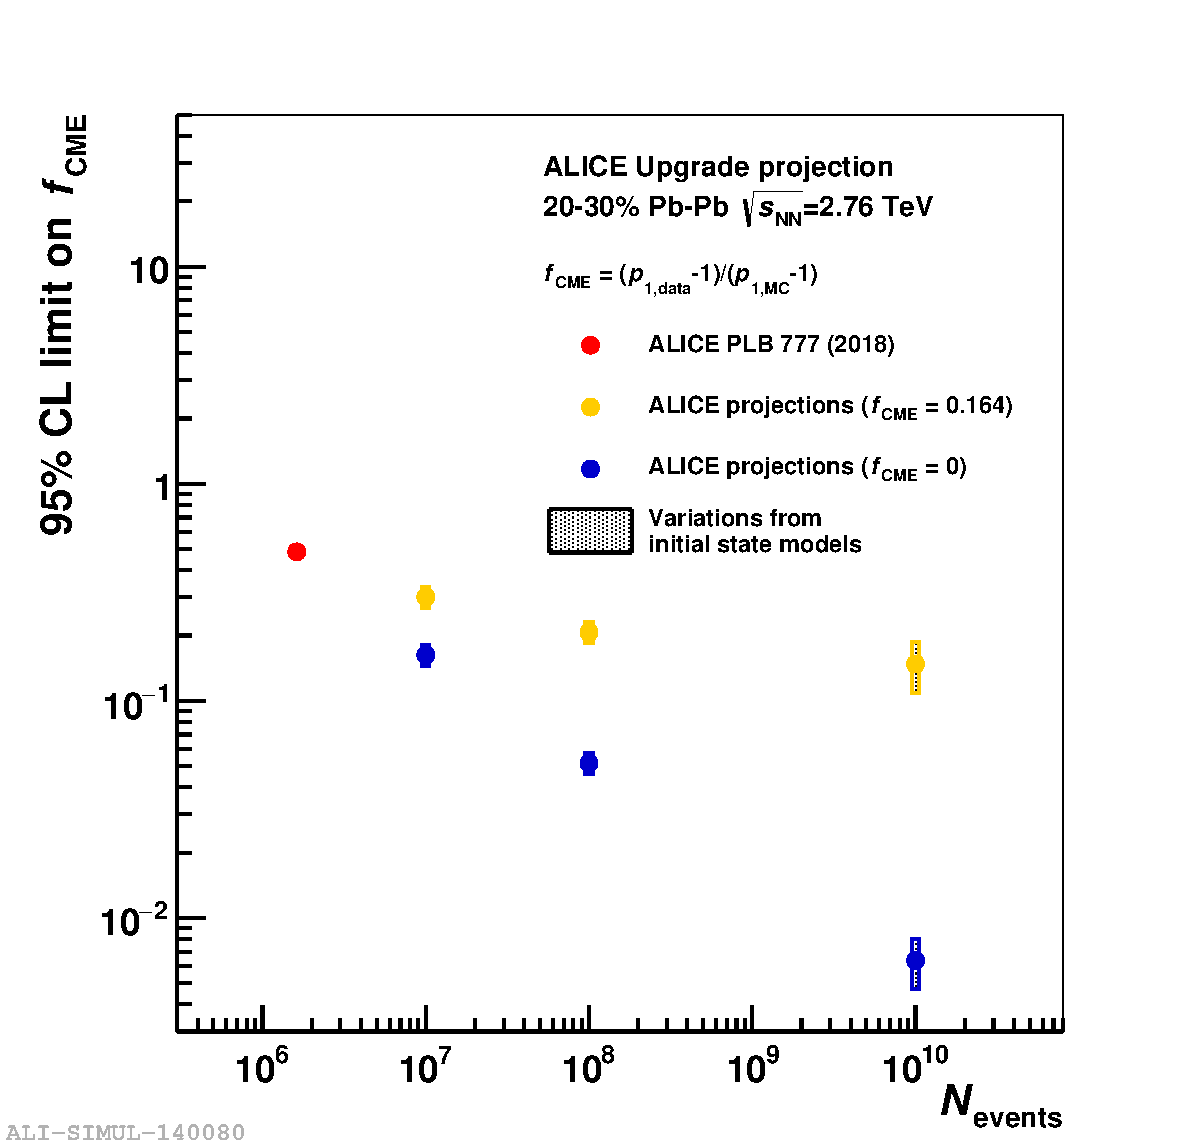
\includegraphics[width=0.6\textwidth]{\main/flow/figs/alice_projection_fcme}
\caption{The upper limit on the CME fraction at 95\% confidence level as a function of the number of events in the 20--30\% centrality interval. The result reported by the ALICE collaboration \cite{Acharya:2017fau} is shown together with expectations for $f_{\rm CME}=0.164$ and $f_{\rm CME}=0$. The shaded boxes denote variations from various initial state models (see text for details).}
\label{fig:alice_fcme}
\end{center}
\end{figure}

The three-particle correlator $\gamma_{\alpha\beta} = \langle \cos(\varphi_{\alpha} + \varphi_{\beta} - 2\Psi_{\rm 2}) \rangle$ \cite{Voloshin:2004vk}, 
where $\varphi_{\alpha}$ is the azimuthal angle of the particle of charge $\alpha$ and $\Psi_{\rm 2}$ is the second harmonic symmetry plane 
angle, was proposed to measure charge-dependent azimuthal correlations. This correlator eliminates correlations independent of symmetry 
plane orientation, suppressing background contributions at the level of $\sim v_2$. However, the interpretation of the experimental results is 
complicated by the remaining background (e.g. local charge conservation (LCC) coupled with elliptic flow~\cite{Schlichting:2010qia, Pratt:2010zn}). 
Recent observation of similar charge-dependent azimuthal correlations in \ppb\ (where the CME is not expected) and 
\pbpb\ collisions~\cite{Khachatryan:2016got} indicates 
the $\gamma_{\alpha\beta}$ correlator be dominated, if not all, by the background effect.
The ALICE \cite{Acharya:2017fau} and CMS \cite{Sirunyan:2017quh} collaborations have used the Event Shape Engineering (ESE) technique 
\cite{Schukraft:2012ah} to estimate the CME fraction to the charge dependence of $\gamma_{\alpha\beta}$, $f_{\rm CME}$, in \pbpb\ collisions. 
ALICE extracted 
$f_{\rm CME}$ by relating measurements of the charge dependence of $\gamma_{\alpha\beta}$ from the ESE analysis to CME signal expectations from 
various initial state model calculations including a magnetic field. It has been assumed that the CME signal is proportional to 
$\langle |B|^2 \cos(2(\Psi_{\rm B} - \Psi_2)) \rangle$, where $|B|$ and $\Psi_{\rm B}$ are the magnitude and direction of the magnetic field, respectively. Within current experimental uncertainties, the CME signal contribution to the $\gamma_{\alpha\beta}$ correlator is consistent with zero.

Figure~\ref{fig:alice_fcme} shows the upper limit on $f_{\rm CME}$ at 95\% confidence level for the 20--30\% centrality interval reported by the 
ALICE collaboration together with expectations for $f_{\rm CME}=0.164$ and $f_{\rm CME}=0$ as a function of the number of events. The shaded 
boxes denote variations due to different estimates of the magnetic field from the investigated models. The ALICE upgrade projection indicates that 
stringent constraints for the CME contribution to the charge dependence of $\gamma_{\alpha\beta}$ can be achieved to a level of less than 1\% 
with the expected HL--LHC statistics. 

One key ingredient needed for the observation of the CME is the strong magnetic field in the QGP medium. It is important to establish a direct
evidence for the presence of this field on final-state particles and to calibrate its strength, which will help significantly constrain theoretical predictions on the magnitude of the CME signal. Measurement of the pseudorapidity-odd component of directed 
flow, $v_1^{\rm odd}$, separately for positive and negative charged particles has been proposed as a probe to 
the magnetic field~\cite{Gursoy:2014aka}. Any difference will indicate the presence of induced electromagnetic 
currents and will allow to estimate the magnitude of the effect. It will also provide information on the electric conductivity of the QGP medium.


\begin{figure}[!htb]
\begin{center}
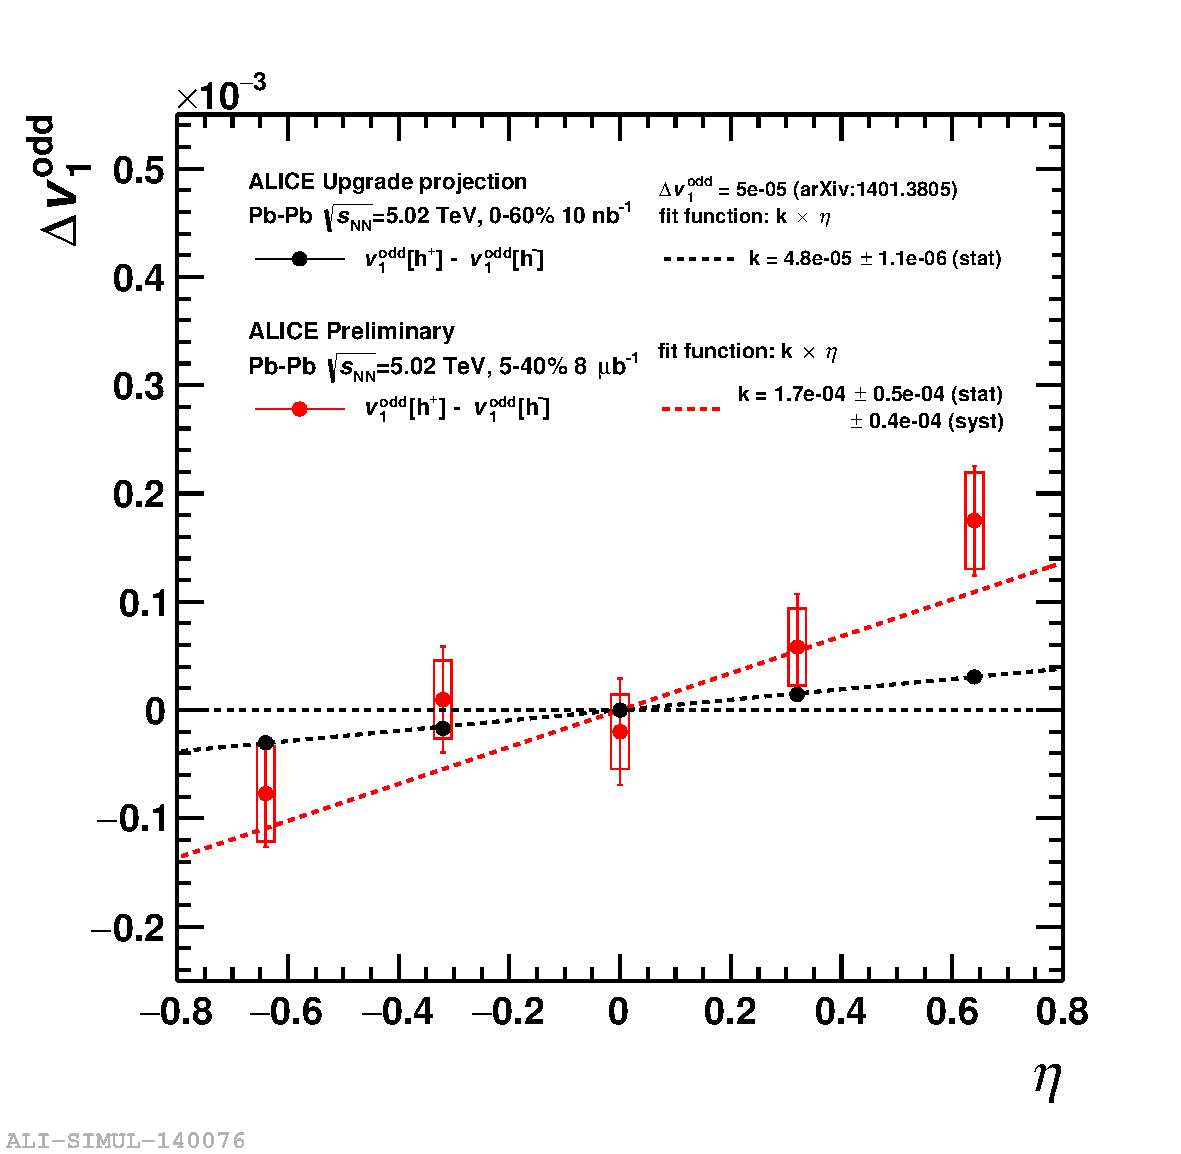
\includegraphics[width=0.6\textwidth]{\main/flow/figs/alice_projection_deltav1ch_stat8}
\caption{Charge difference of $v_1^{\rm odd}$ as a function of pseudorapidity measured by the ALICE collaboration in \pbpb\ collisions at $\snn=5.02$ TeV  \cite{Margutti:2017lup} (red symbols) and the expectation for a $5 \times 10^{-5}$ difference \cite{Gursoy:2014aka} from 10 nb$^{-1}$ (black symbols) together with linear fits (dashed lines). Error bars (open boxes) represent the statistical (systematic) uncertainties.}
\label{fig:alice_delta_v1}
\end{center}
\end{figure}


Figure~\ref{fig:alice_delta_v1} shows the charge difference of $v_1^{\rm odd}$, 
$\Delta v_1^{\rm odd}=v_1^{\rm odd +} - v_1^{\rm odd -}$, as a function of pseudorapidity measured by the ALICE collaboration in Pb--Pb collisions 
at $\snn=5.02$ TeV \cite{Margutti:2017lup} together with a linear fit. A hint of a charge-dependent difference is observed and quantified 
by the slope $k$ with a total significance of 2.6 $\sigma$. This difference, which differs both in magnitude and sign compared to predictions for 
$\pi^{\pm}$ at $\snn=2.76$ TeV and similar $\langle p_{\rm T} \rangle$ \cite{Gursoy:2014aka}, needs to be confirmed. 
This will be achieved 
with the large data sample expected at the HL--LHC where even the predicted difference of $5 \times 10^{-5}$ will be measured with high accuracy 
as reported by the ALICE upgrade projection in Fig. \ref{fig:alice_delta_v1}. Furthermore, similar measurement can also be performed
in the heavy flavor sector, e.g., for $D^{0}$ and $\overline{D^{0}}$ meson directed flow~\cite{Das:2016cwd}. Heavy flavor quarks have the advantage of
being produced at a very early stage, and thus potentially have a better sensitivity to the magnetic field at its peak magnitude before it decays.




